% !TeX spellcheck = ru_RU
% !TeX encoding = UTF-8
\section{Технология Lonta Optima}
\subsubsection{Назначение}
Радиоканальная система пультовой охраны Lonta Optima компании «Альтоника» предназначена для централизованной охраны территориально распределенных стационарных объектов с передачей охранно-пожарных извещений по радиоканалу.
\subsubsection{Структура системы}
Рассмотрим структуру системы Lonta Optima. Типичная сеть Lonta Optima состоит из следующих элементов: 
\begin{itemize}
	\item"Датчики". В технологии Lonta Optima "датчиками" являются приемно-контрольные приборы со встроенным передатчиком.  
	\item"Приёмники". В технологии  Lonta Optima используется термин "выносной приемник".
	\item"Пункт сбора". В технологии  Lonta Optima "пунктом сбора" является пульт централизованного наблюдения. В большинстве случаев пульт централизованного наблюдения подключается к компьютеру с программным обеспечением рабочего места оператора(по полученным данным производится охранный мониторинг), но может использоваться и автономно.  
\end{itemize}

Структурная схема системы представлена на рисунке
\ref{fig:Lonta_Optima}.

\begin{figure}[H]
	\centering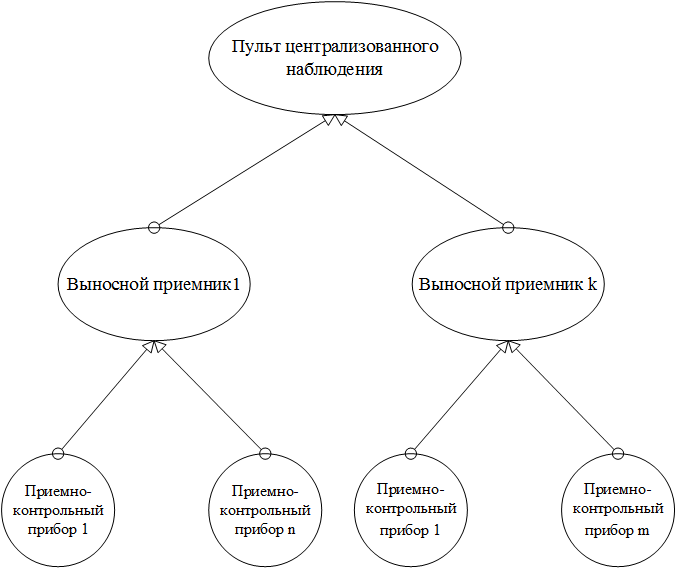
\includegraphics[width=0.7\linewidth]{img/Lonta_Optima}
	\caption{Структурная схема системы, построенной по технологии Lonta Optima}
	\label{fig:Lonta_Optima}
\end{figure}

В состав системы с одним пультом может входить до 500 передатчиков.

В системе Lonta Optima базовая станция и передатчики работают на определенном наборе частот в пределах разрешенной полосы 433,92 МГц. Этот набор частот называется «частотная литера». Всего в разрешенной полосе частот можно при необходимости разместить до 36 неперекрывающихся литер.
В одном городе или районе на разных частотных литерах одновременно могут работать до четырех систем Lonta Optima.

\textbf{Особенности:}
\begin{itemize}

\item Дальность связи составляет до 10 км в условиях городской застройки и до 25 км за городом.
\item Контроль связи с каждым объектом - 20-90 минут (устанавливается пользователем).
\item На одной территории возможно одновременное использование 2000 передатчиков на 4 частотных литерах.
\end{itemize}

\subsubsection{Разбиение системы на уровни}
Способ разбиения системы  Lonta Optima на уровни представлен на рисунке
\ref{fig:system_levels}.
\begin{figure}[H]
	\centering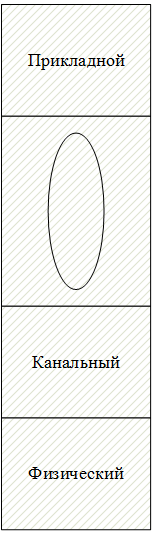
\includegraphics[width=0.2\linewidth]{img/system_levels}
	\caption{Разбиение на уровни системы Lonta Optima}
	\label{fig:system_levels}
\end{figure}

\subsubsection{Особенности построения уровней}
Главной особенностью построения уровней системы  Lonta Optima является то, что все уровни данной системы являются закрытыми.

\textbf{Особенности физического уровня системы:}

\begin{itemize}
	
	\item Для эксплуатации системы не требуется получение разрешения на использование радиочастоты.
	\item Система работает на открытой частоте 433,92 МГц.
	\item Мощность объектовых передатчиков составляет 10 мВт\cite{3}.
	
\end{itemize}

\newpage